\documentclass[12pt]{article}

% Packages
\usepackage[utf8]{inputenc}
\usepackage{xeCJK}
\usepackage{ctex}
\usepackage{amsmath, amssymb}
\usepackage{graphicx}
\usepackage{hyperref}
\usepackage{geometry}
\usepackage{float}
\usepackage{cite}
\usepackage{subcaption}

% Page layout
\geometry{a4paper, margin=1in}

% Title and Author
\title{基于BSSMF矩阵分解的图像降噪方法}
\author{王伟钊}
\date{\today}

\begin{document}

\maketitle

\begin{abstract}

\end{abstract}

\tableofcontents

\section{绪论}
随着信息时代的快速发展,数字图像处理技术在各个领域得到了广泛的应用。然而,由于图像采集设备的限制,图像中常常会受到各种形式的噪声干扰。图像降噪是图像处理中的一个重要问题,其目的是去除图像中的噪声,使图像更加清晰,便于后续的图像分析和处理。图像降噪技术在医学图像处理、卫星图像处理、安防监控等领域有着广泛的应用。

\subsection{问题描述}
在数学上,图像降噪问题可以用如下数学表达式描述\cite{SVDWhiteNoise}:
\begin{equation}
    A(i,j)=A_{0}(i,j)+N(i,j)
\end{equation}
其中$A(i,j)$是观测到的图像,$A_{0}(i,j)$是原始图像,$N(i,j)$是噪声。噪声$N(i,j)$可以是各种形式的,图\ref{fig:noise_types}展示的是最常见的两种噪声:高斯白噪声和椒盐噪声。
\begin{figure}[H]
    \centering
    % 子图 (a)
    \begin{subfigure}[b]{0.45\textwidth}
        \centering
        
\includegraphics[width=\textwidth]{images/Gaussian_noise.png}
        \caption{高斯白噪声,$\mu$=0,$\sigma^2$=30}
    \end{subfigure}
    \hfill
    % 子图 (b)
    \begin{subfigure}[b]{0.45\textwidth}
        \centering
        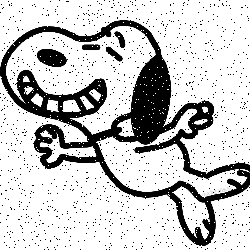
\includegraphics[width=\textwidth]{images/salt_pepper_noise.png}
        \caption{椒盐噪声}
    \end{subfigure}
    \caption{高斯白噪声和椒盐噪声}
    \label{fig:noise_types}
\end{figure}

本文主要关注高斯白噪声的降噪问题。高斯白噪声是一种均值为0,方差为$\sigma^2$的高斯分布,其概率密度函数为:

\begin{equation}
    f(x)=\frac{1}{\sqrt{2\pi}\sigma}e^{-\frac{(x - \mu)^{2}}{2\sigma^{2}}}
\end{equation}
其中$\mu$是均值,$\sigma$是标准差。由于大部分的白噪声均值为0,因此估计$\sigma$成为了图像降噪中的一个关键步骤,因为它直接影响降噪算法的性能。准确估计噪声水平可以帮助选择合适的降噪参数,从而在保留图像细节和去除噪声之间取得平衡。如果$\sigma$估计不准确,可能会导致过度平滑(损失细节)或降噪不足(残留噪声)\cite{Estimation_of_noise_variance}。为此,K. Rank等人\cite{MADestimate}使用绝对中位差(MAD)方法进行估计,Fabrizio Russo等人\cite{AWGN}在2003年提出了一种基于新型滤波器对标准差$\sigma$进行估计的方法。Liu等人在2013年提出了基于SVD的方法\cite{SVDWhiteNoise}进行估计。有了准确的噪声估计,我们就可以选择合适的降噪算法对图像进行降噪。

\subsection{国内外降噪算法研究现状}
\subsubsection{基于传统滤波器的方法}
\subsubsection{基于小波变换的方法}
\subsubsection{基于深度学习的方法}

\section{相关工作}

\section{实验设计}

\section{实验结果与分析}

\section{结论}

\bibliographystyle{plain}
\bibliography{ref}

\appendix
\section{Appendix}
Include additional material, derivations, or data that support your paper but are not essential to the main text.


\end{document}